%% ****** Start of file apstemplate.tex ****** %
%%
%%
%%   This file is part of the APS files in the REVTeX 4 distribution.
%%   Version 4.1r of REVTeX, August 2010
%%
%%
%%   Copyright (c) 2001, 2009, 2010 The American Physical Society.
%%
%%   See the REVTeX 4 README file for restrictions and more information.
%%
%
% This is a template for producing manuscripts for use with REVTEX 4.0
% Copy this file to another name and then work on that file.
% That way, you always have this original template file to use.
%
% Group addresses by affiliation; use superscriptaddress for long
% author lists, or if there are many overlapping affiliations.
% For Phys. Rev. appearance, change preprint to twocolumn.
% Choose pra, prb, prc, prd, pre, prl, prstab, prstper, or rmp for journal
%  Add 'draft' option to mark overfull boxes with black boxes
%  Add 'showpacs' option to make PACS codes appear
%  Add 'showkeys' option to make keywords appear
\documentclass[aps,pre,twocolumn,groupedaddress]{revtex4-1}
%\documentclass[aps,pre,preprint,superscriptaddress]{revtex4-1}
%\documentclass[aps,prl,reprint,groupedaddress]{revtex4-1}

% You should use BibTeX and apsrev.bst for references
% Choosing a journal automatically selects the correct APS
% BibTeX style file (bst file), so only uncomment the line
% below if necessary.
\bibliographystyle{apsrev4-1}

\usepackage{graphicx}
\usepackage{amsmath}

\begin{document}

% Use the \preprint command to place your local institutional report
% number in the upper righthand corner of the title page in preprint mode.
% Multiple \preprint commands are allowed.
% Use the 'preprintnumbers' class option to override journal defaults
% to display numbers if necessary
%\preprint{}

%Title of paper
\title{Bulk Flow Behaviour of Cubic Blue Phases}

% repeat the \author .. \affiliation  etc. as needed
% \email, \thanks, \homepage, \altaffiliation all apply to the current
% author. Explanatory text should go in the []'s, actual e-mail
% address or url should go in the {}'s for \email and \homepage.
% Please use the appropriate macro foreach each type of information

% \affiliation command applies to all authors since the last
% \affiliation command. The \affiliation command should follow the
% other information
% \affiliation can be followed by \email, \homepage, \thanks as well.
\author{O. Henrich$^{1,3}$, K. Stratford$^2$, D. Marenduzzo$^3$, P.V. Coveney$^1$ and M.E. Cates $^3$}
\affiliation{$^1$ Centre for Computational Science, University College London, UK\\$^2$ Edinburgh Parallel Computing Centre, University of Edinburgh, UK\\$^3$ School of Physics and Astronomy, University of Edinburgh, UK}

%\email[]{}
%\homepage[]{Your web page}
%\thanks{}
%\altaffiliation{}

%Collaboration name if desired (requires use of superscriptaddress
%option in \documentclass). \noaffiliation is required (may also be
%used with the \author command).
%\collaboration can be followed by \email, \homepage, \thanks as well.
%\collaboration{}

%\noaffiliation

\date{\today}

\begin{abstract}
\end{abstract}

% insert suggested PACS numbers in braces on next line
\pacs{}
% insert suggested keywords - APS authors don't need to do this
%\keywords{}

%\maketitle must follow title, authors, abstract, \pacs, and \keywords
\maketitle

% body of paper here - Use proper section commands
% References should be done using the \cite, \ref, and \label commands
\section{Introduction}
% Put \label in argument of \section for cross-referencing
%\section{\label{}}
\section{Model and Methods}

Our approach is based on a well-established model for hydrodynamics of cholesteric liquid crystals \cite{Beris:1994,Olmsted:1999} that describes the order structure of the liquid crystal by a traceless, symmetric tensor order parameter ${\bf Q}({\bf r})$. 
In uniaxial approximation the tensor order paramter is given by $Q_{\alpha \beta}=\langle n_\alpha n_\beta - 1/3\; \delta_{\alpha\beta}\rangle$, whereas ${\bf n}$ represents the local orientation of the liquid crystal molecules and brackets indicate mesoscopic averaging over a large number individual molecules.
Its largest eigenvalue $\frac{2}{3}q$ with $0<q<1$ characterizes the degree of order around the corresponding axis. 
The equilibrium properties of the system are determined by a Landau-de Gennes free energy density $f$ and the functional ${\cal F}[Q]=\int d^3{\bf r} f({\bf Q})$.
The free energy density consists of two different parts, namely a bulk contribution $f_b$ and a gradient term $f_g$.

\begin{eqnarray}
f_b&=&\frac{A_0}{2}\left(1-\frac{\gamma}{3}\right) Q_{\alpha \beta}^2-\frac{A_0 \gamma}{3}Q_{\alpha \beta} Q_{\beta \gamma} Q_{\gamma \alpha}+\frac{A_0 \gamma}{4}(Q_{\alpha \beta}^2)^2\nonumber\\
f_g&=&\frac{K}{2}(\varepsilon_{\alpha\gamma\delta} \partial_\gamma Q_{\delta\beta}+2 q_0 Q_{\alpha \beta})^2+\frac{K}{2}(\partial_\beta Q_{\alpha \beta})^2\label{eqn1}
\end{eqnarray}

The first term contains the bulk-free energy constant $A_0$ and the inverse temperature $\gamma$ and features a the first-order transition from the isotropic to the ordered phase at $\gamma>2.7$.
The second part comprises the elastic contributions to the free energy due to splay-, bend- and twist-deformations and assume for simplicity that they have all the same elastic constant $K$.
The pitch length $p$ of the cholesteric liquid crystal is related to the wavervector $q_0=2\pi/p$.
In order to specify a thermodynamic state it is useful to introduce two dimensionless quantities, the effective temperature $\tau$ and chirality $\kappa$.
They are given by 

\begin{eqnarray}
\tau&=&\frac{27(1-\gamma/3)}{\gamma}\nonumber\\
\kappa&=&\sqrt{\frac{108 K q_0^2}{A_0 \gamma}}\nonumber,
\end{eqnarray}

whereas the chirality qqnatifies the ratio between gradient and bulk free energy.\\
The equation of motion of the tensor order parameter reads

\begin{equation}\label{}
\left(\partial_t+ u_\alpha \partial_\alpha \right){\bf Q} - {\bf S}({\bf W},{\bf Q}) = \Gamma {\bf H}.
\label{eqn2}
\end{equation}

The first term on the lefthand side of Eq.(\ref{eqn2}) is a material derivative, which describes the rate of change of a quantity moving along with the flow.
The second term accounts for the rate of change due to velocity gradients $W_{\alpha \beta}=\partial_\beta u_\alpha$:

\begin{eqnarray}
{\bf S}({\bf W}, {\bf Q}) &=& (\xi {\bf A} + {\boldsymbol \Omega})({\bf Q}+\frac{\bf I}{3})\nonumber\\
& &\hspace*{-1.5cm}+ ({\bf Q}+\frac{\bf I}{3})(\xi {\bf A}  - {\boldsymbol \Omega})-2 \xi ({\bf Q}+\frac{\bf I}{3})Tr({\bf Q W}),
\label{eqn3}
\end{eqnarray}

where $Tr$ denotes the trace operation and ${\bf A}=({\bf W}+{\bf W}^T)/2$ and ${\boldsymbol \Omega}=({\bf W}-{\bf W}^T)/2$ are the symmetric and antisymmetric part of the velocity gradients, respectively.
The molecular details of the liquid crystal such as the aspect ratio of its mesogens are embodied in the constant $\xi$, also know as the tumbling parameter.
The righthand side relates the rate of change to the molecular field, which is a functional derivative of $\cal F$ that preserves the tracelessness of $\bf Q$.

\begin{equation}
{\bf H}=-\frac{\delta {\cal F}}{\delta {\bf Q}}+\frac{\bf I}{3}\, Tr\left(\frac{\delta {\cal F}}{\delta {\bf Q}}\right).
\label{eqn4}
\end{equation}

The rotational diffusion constant $\Gamma$ is proportional to the inverse of the rotational viscosity $\gamma_1=2 q^2/\Gamma$.\\
The time evolution of density and velocity are goverend by the continuity equation Eq. (\ref{eqn5}) 

\begin{eqnarray}
\partial_t \rho + \partial_\alpha (\rho u_\alpha)=0
\label{eqn5}
\end{eqnarray}

and the Navier-Stokes equation Eq. (\ref{eqn6})

\begin{eqnarray}
\partial_t u_\alpha +\rho \,u_\beta \partial_\beta u_\alpha&=&\partial_\beta \Pi_{\alpha \beta}\nonumber\\
&+&\hspace*{-2cm}\eta\, \partial_\beta \{ \partial_\alpha u_\beta + \partial_\beta u_\alpha +(1+3\frac{P_0}{\partial \rho} )\partial_\mu u_\mu \delta_{\alpha \beta})\}. 
\label{eqn6}
\end{eqnarray}

At low flow rates the fluid can be considered as incompressible, so that the last term on the righthand side of Eq. (\ref{eqn6}) can be safely neglected.
The pressure tensor reads explicitely

\begin{eqnarray}
\Pi_{\alpha \beta}&=&P_0-\xi H_{\alpha \gamma}\left(Q_{\gamma \beta} +\frac{1}{3} \delta_{\gamma \beta}\right)-\xi \left(Q_{\alpha \gamma} +\frac{1}{3} \delta_{\alpha \gamma}\right) H_{\gamma \beta}\nonumber\\
&+& 2 \xi  \left(Q_{\alpha \beta} +\frac{1}{3} \delta_{\alpha \beta}\right) Q_{\gamma \nu} H_{\gamma \nu}-\partial_\alpha Q_{\gamma \nu} \frac{\delta{\cal F}}{\delta \partial_{\beta} Q_{\gamma \nu}}\nonumber\\
&+&Q_{\alpha \gamma}H_{\gamma \beta}-H_{\alpha \gamma} Q_{\gamma \beta}.
\label{eqn7}
\end{eqnarray}

It comprises the terms that give rise to an additional stress in the ordered state.
In the isotropic state when ${\bf Q}\equiv 0$ Eq. (\ref{eqn7}) is reduced to the scalar pressure, which is constant to a very good approximation.\\ 
The system of coupled partial differential equations is solved by means of a hybrid scheme \cite{Denniston:2004, Marenduzzo:2008} that uses a lattice Boltzmann algorithm with predictor-corrector scheme for the hydrodynamic equations (\ref{eqn5}) and (\ref{eqn6}) and a finite difference scheme for the tensor order parameter equation (\ref{eqn2}).


\section{Results and Discussion}

In the following we report results on the bulk flow behaviour of BPI and BPII for thermodynamic states characterized by $\tau=-0.5$ and $\kappa=1.0$ (BPI) and $\kappa=2.0$ (BPII), respectively.
For these parameters both blue phases are equilibrium phases in the quiescent state.
We have also performed simulations at higher temperatures and chiralities and for metastable configurations, which led to very similar results.
Quantitative differences occured only in that sense that the disclination network dissolved more easily for a particular flow rate if the system was closer to the cholesteric-isotropic phase boundary and where the order parameter takes lower values and free energy density is higher.\\
The tensor order parameter was initialized with the high-chirality solution of Eq. \ref{eqn1}, which has the correct topology of the actual blue phase.
The initial configurations were equilibrated for $5000$ LB time steps, where we allowed for optimization of the unit cell size \cite{Alexander:2006}, a feature that is often referred to as 'redshift'.
After the equilibration sequence the unit cell size was fixed and the shear flow was switched on.
For BPII we used a pitch length of 32 lattice sites, but in case of BPI it was necessary to increase the resolution to 64 sites per pitch length to get accurate results of the flow induced transformations in the disclination network.
In order to impose a flow profile we used Lees-Edwards boundary conditions \cite{Wagner:2002}, whereas the top (bottom) half of planes moved in positive (negative) y-direction.
We applied a correction for spurious momentum currents that emerge due to interpolations accross the Lees-Edwards planes \cite{Henrich:2011b}.
The imposed flow rates ranged over two orders of magnitude from about $1.25\cdot 10^{-6}$ to $6\cdot10^{-4}$ in LB units.\\
In the visualizations that follow the orientation of the principal coordinate axes in x-, y- and z-direction always coincides with the direction of the velocity gradient direction, the flow and the vorticity, respectively.
Disclination lines are plotted as isosurface of the scalar order parameter $q$

\subsection{Blue Phase II}

We start the discussion with BPII, because its flow behaviour is simpler and probably more easily anticipated.
Fig \ref{fig1} shows the disclination network undergoing a flow-induced transformation.
The periodically recurring structure remains very regular and apart from the quasi-affine transformation relatively close to its quiescent appearance with individual disclination lines breaking up and reconnecting further downstream.

\begin{figure*}[h]
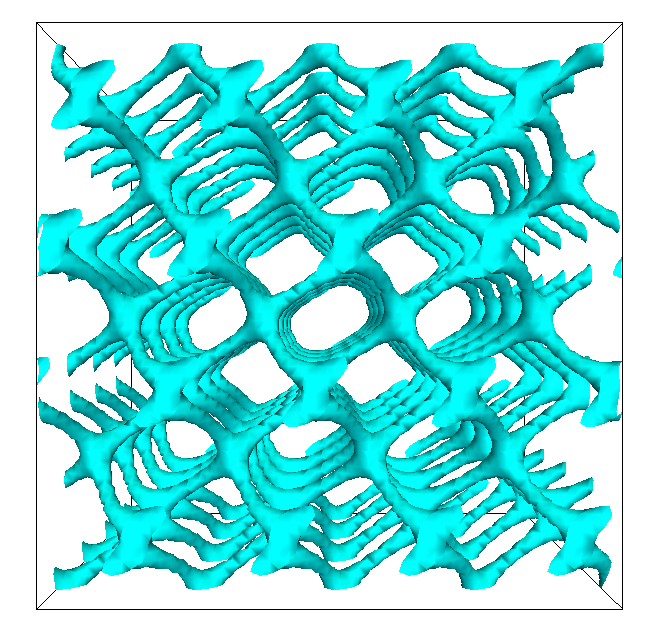
\includegraphics[width=0.32\textwidth]{disc-160k_run902.png}
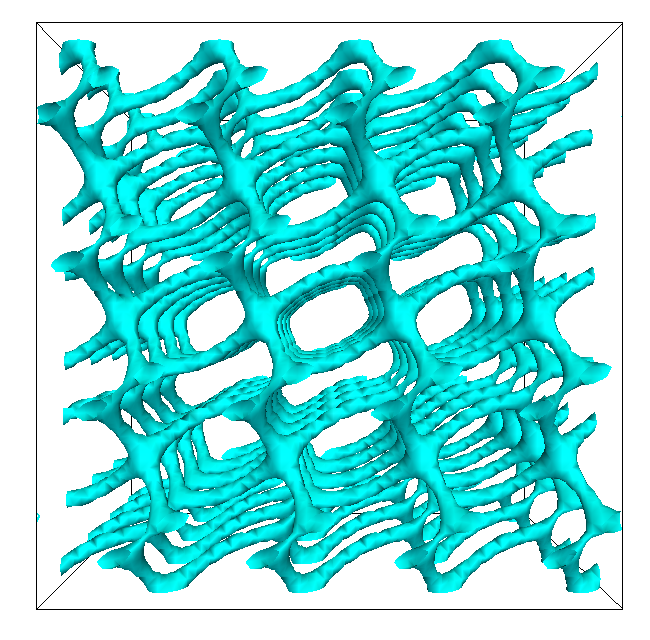
\includegraphics[width=0.32\textwidth]{disc-164k_run902.png}
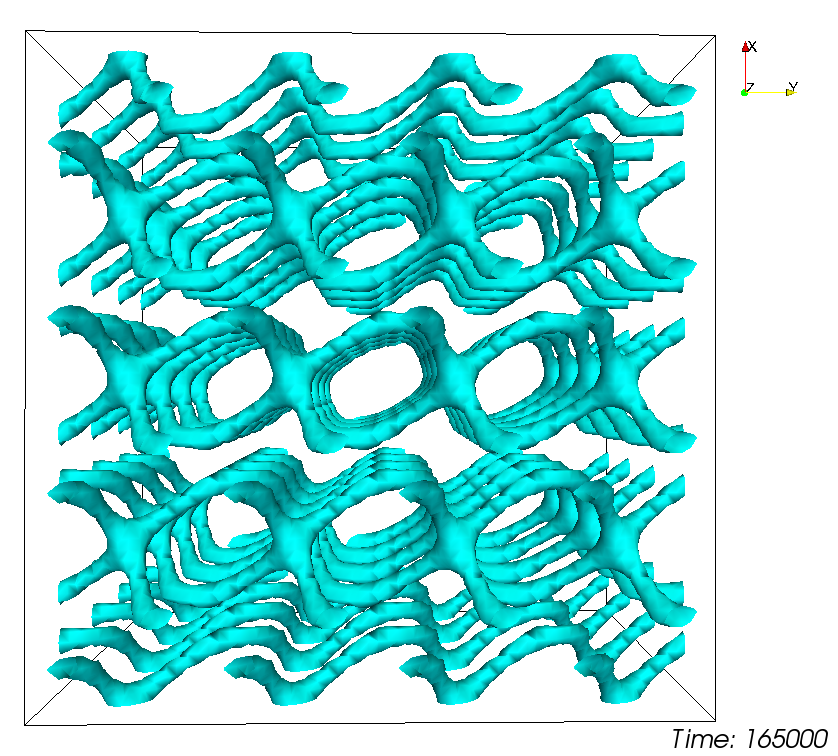
\includegraphics[width=0.32\textwidth]{disc-165k_run902.png}
\caption{Disclination network of BPII in shear flow: The pictures show a typical sequence of shear-induced transformations in the steady state at $\dot{\gamma}=1.56\cdot 10^{-4}$. The horizontal y-direction is the flow direction whereas the velocity gradient is oriented along the vertical x-direction.}
\label{fig1}
\end{figure*}

Interestingly, while being steadily sheared in y-direction, the entire disclination network is slowly displaced in z-direction, the direction of vorticity.
This feature is most clearly observed when the structure is viewed along the flow direction.
Fig. \ref{fig2} depicts a sequence of close-ups of the disclination network as it travels in negative z-direction, i.e. from the foreground towards the background of the picture. 
The velocity $v_z$, represented by the colour code, exhibits a recurring pattern of positive and negative values.
Peak velocities occur close to disclination lines where the molecular order is suppressed or in regions where two disclination lines approach each other and the network is about to break up or reform. 

\begin{figure*}[h]
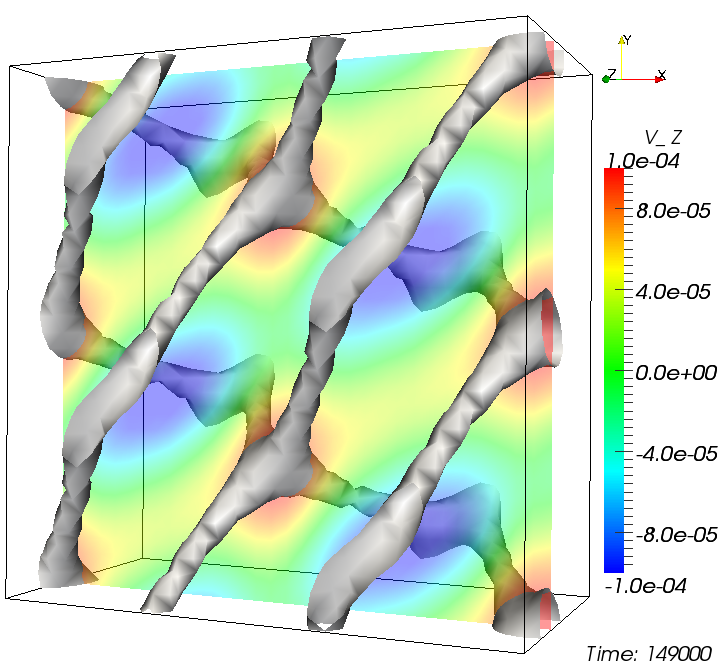
\includegraphics[width=0.32\textwidth]{slice-disc-v_z-149k_run902.png}
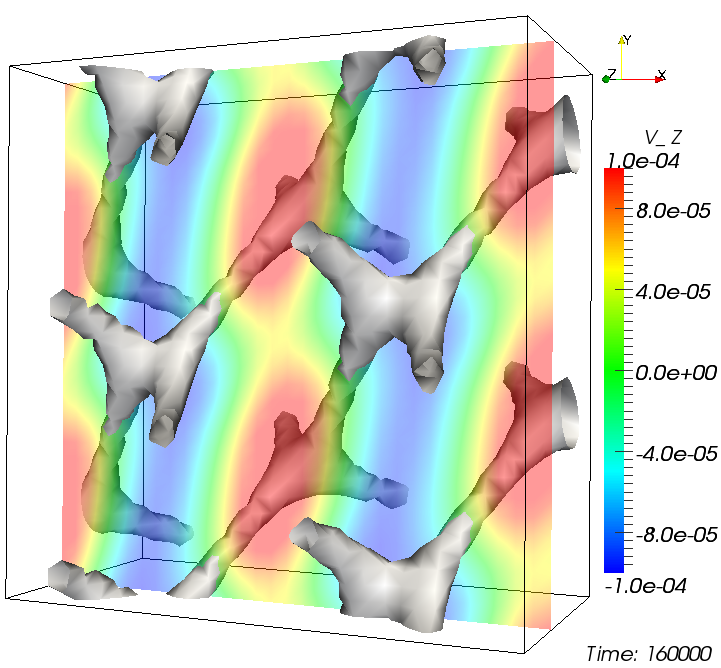
\includegraphics[width=0.32\textwidth]{slice-disc-v_z-160k_run902.png}
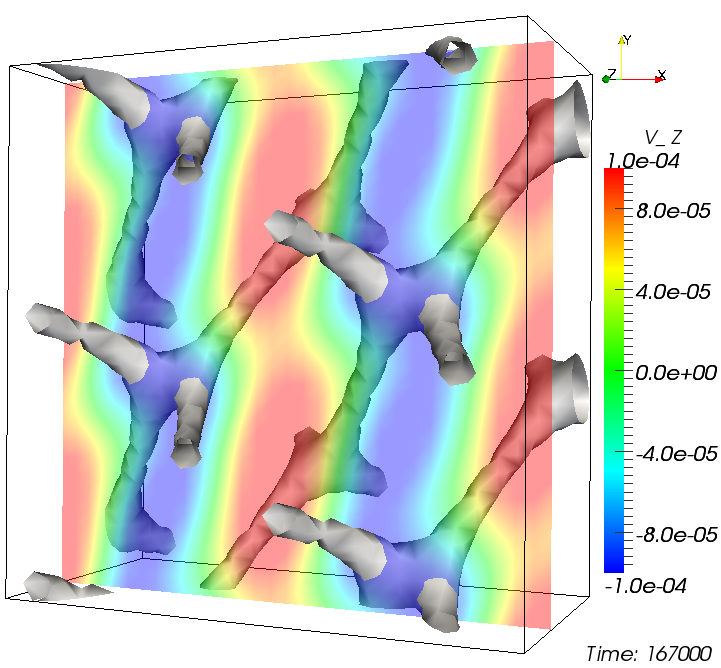
\includegraphics[width=0.32\textwidth]{slice-disc-v_z-167k_run902.png}\\
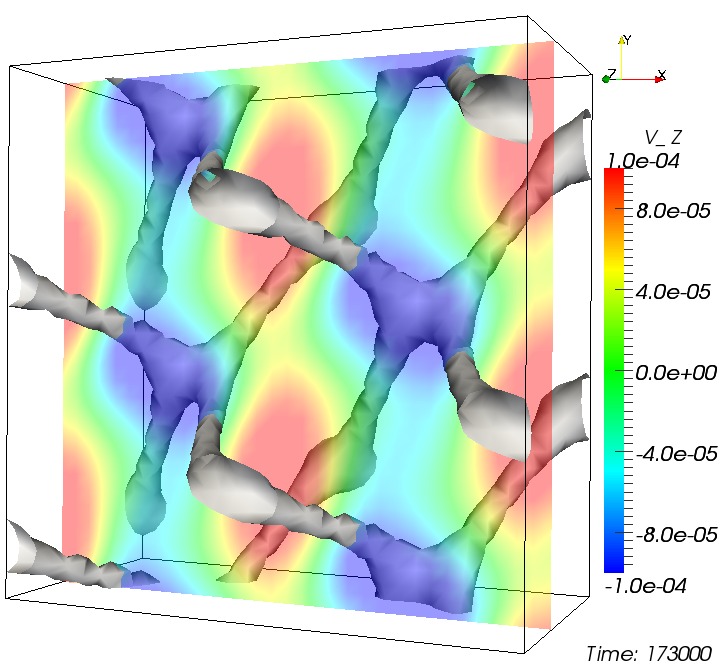
\includegraphics[width=0.32\textwidth]{slice-disc-v_z-173k_run902.png}
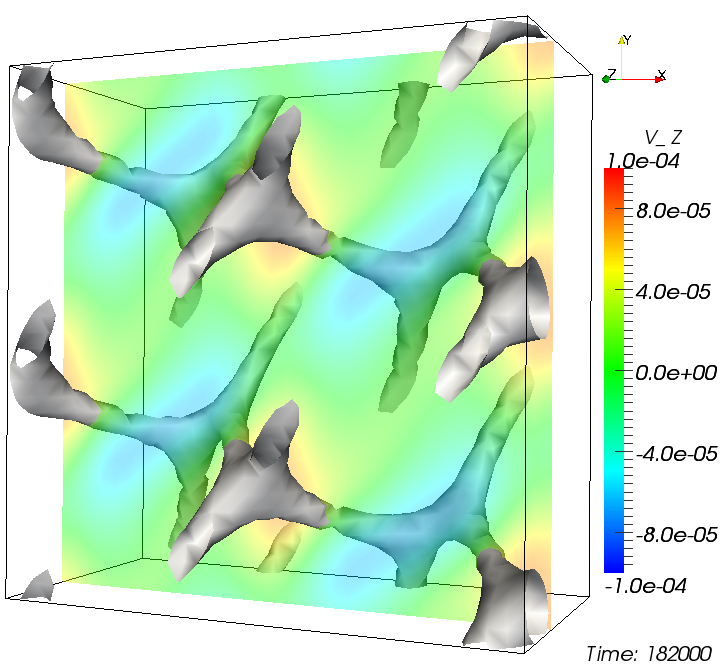
\includegraphics[width=0.32\textwidth]{slice-disc-v_z-182k_run902.png}
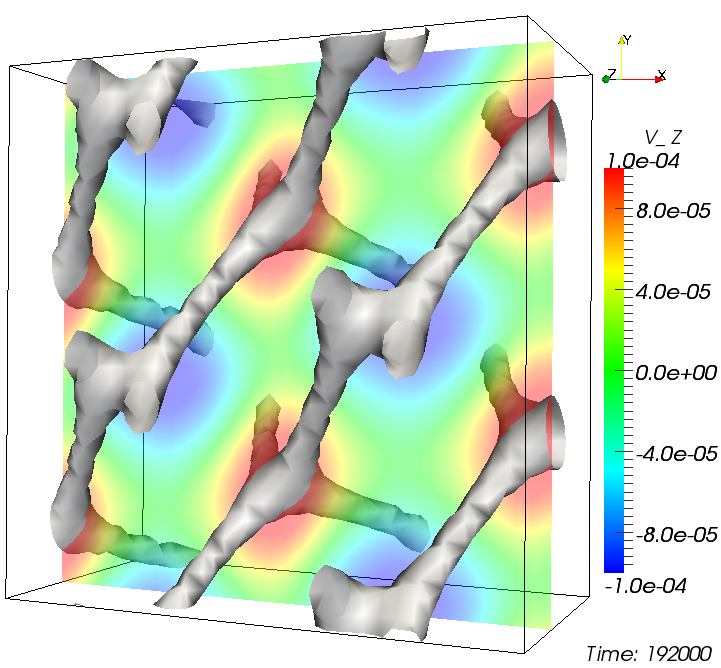
\includegraphics[width=0.32\textwidth]{slice-disc-v_z-192k_run902.png}\\
\caption{A section of $2\times2\times1$ unit cells of BPII seen along the direction of vorticity. The colour code gives the magnitude and direction of the velocity component $v_z$ perpendicular to the plane.}
\label{fig2}
\end{figure*}

Plotting only x- and z-component of the local velocity allows to visualize the spatial dependence of the secondary flow in the blue phase with respect to the disclination network.
Fig. \ref{fig3} shows characteristic regions of upward and downward 'flow', which are normally superimposed by the primary shear flow in y-direction.
Remarkably, the secondary flow is directly connected to the sense of the underlying cholesteric helix as changing from left- to right-handed helix also inverts the sense of motion of the network.
%%%-----%%%%%%%%%%%

The lefthand picture depicts the situation the movement of the disclination network is downwards, while helix inversion leads to an upward motion in the righthand picture.
More precisely the orientation of the velocities with respect to the bands is exactly inverted in both cases. 

A closer look at the shape of the disclination lines reveals that also the network seems to be inverted. 
The total magnitude of the secondary flow is in the range of a few percent of the primary flow and the images in Fig. \ref{fig3} give actually the situation close to the peak point.\\ 

A secondary flow pattern with distinctive regions of positive and negative velocity components $v_z$ emerges and reoccurs periodically.



\begin{figure*}[h]
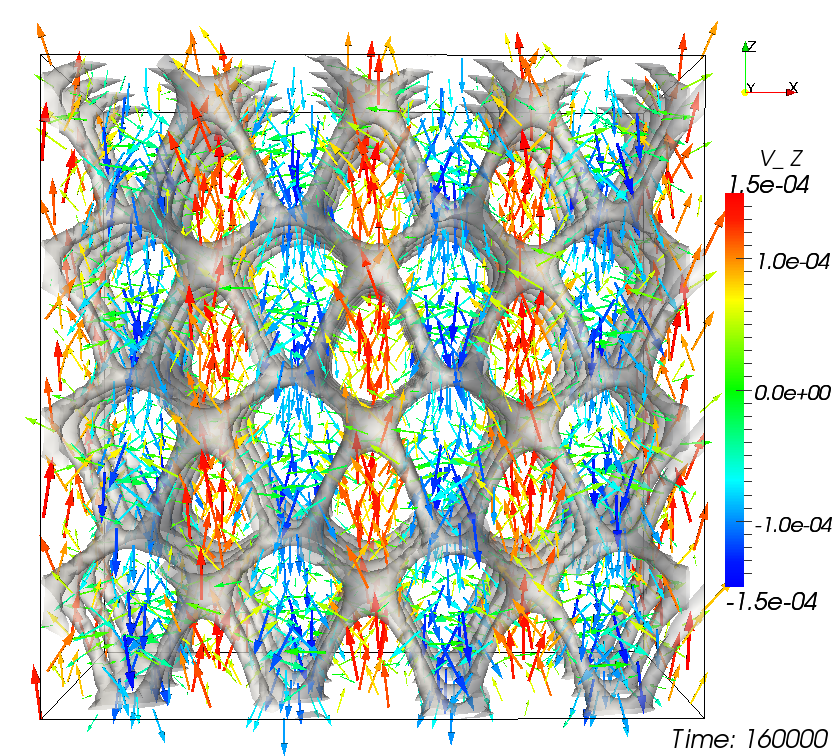
\includegraphics[width=0.45\textwidth]{v_xz-v_z-160k_run902.png}
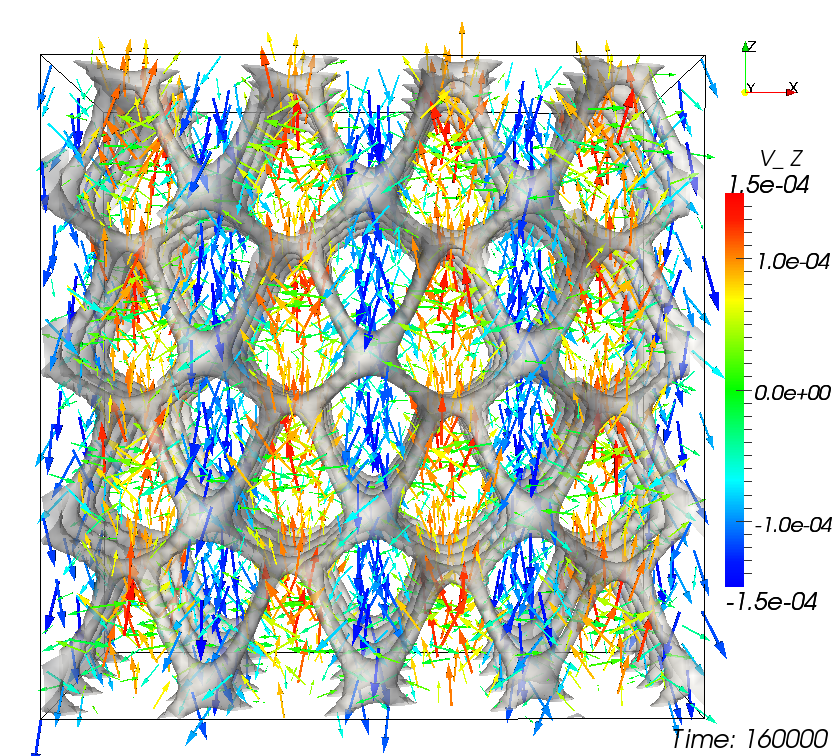
\includegraphics[width=0.45\textwidth]{v_xz-v_z-160k_run903.png}
\caption{Secondary flow in BPII visualized by means of the velocity components $v_x$ and $v_z$ for positive (left) and negative (right) helicity of the cholesteric helix. The images depict an individual snapshot of the periodically recurring sequence in the steady state.}
\label{fig3}
\end{figure*}


It is interesting to study the flow behaviour from a more quantitative point of view by looking at the shear stress dependence on flow rate and time. 

The effective viscosity $\eta_{eff}$ over time is shown in Fig. \ref{fig4}. 
For all apart from the highest flow rate it oscillates sinusoidally, exhibiting symmetric minima and maxima and decreasing mean values, indicating slightly shear-thinning behaviour.
The period reflects the time it takes for the disclination network to break up and reconnect as shown in Fig. \ref{fig1}.
However, due to the motion of the network in z-direction it turns out that it takes four periods altogether for the network to move one unit cell along the direction of vorticity and to complete one cycle.
The inset shows the deviatoric part of the chemical stress tensor as a function of shear rate.
The dependence is that of a power law $\sigma_{eff, xy}=a \dot{\gamma}^b$ with $a=0.34(6116), b=0.95(2654)$ for low and intermediate shear rates. 
The error bars indicate the maximum and minimum stress during one cycle.
The idependence is almost linear and gives further evidence of the remarkably small degree of shear-thinning and also reflected in the very regular and undisturbed affine transformation of the disclination network.  

\begin{figure}[h]
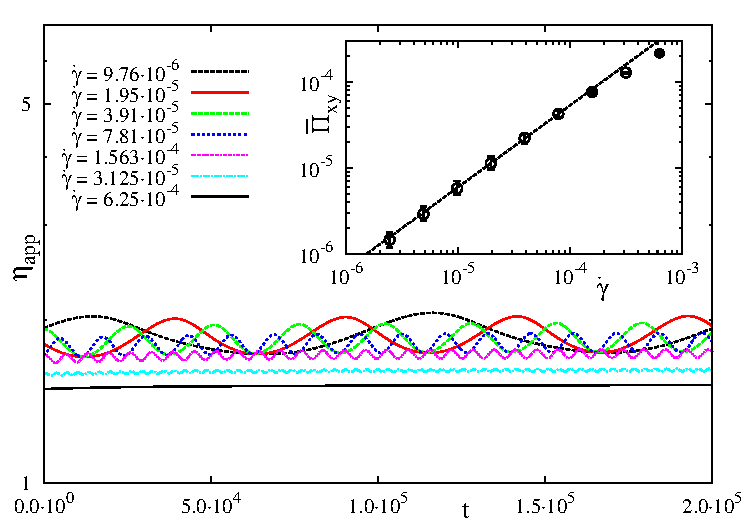
\includegraphics[width=0.5\textwidth]{stress_bp2.pdf}
\caption{Effective viscosity $\eta_{eff}=\Sigma_{xy}/\dot{\gamma}$ over time and flow curve $\sigma_{chem}(\dot{\gamma})$ (inset) of BPII in the steady state. }
\label{fig4}
\end{figure}

Above a critical shear rate, which is $\dot{\gamma}=3.1-6.2\cdot 10^{-4}$ in our case, the rotational diffusion coefficient $\Gamma$ in Eq. \ref{eqn2} is too small and the disclination network adopts a completely different conformation in the steady state.
Fig. \ref{fig5} shows the director field and the position of disclination plane.
The degree of twist is the same as that of the underlying cholesteric, but the orientation of the director on either side of the planes differs by almost 90 degrees, giving rise to four distinct layers, which are separated by disclination planes.
Even in this flow-induced state the disclinations move and retain the above described sense of motion in the direction of vorticity.

\begin{figure}[h]
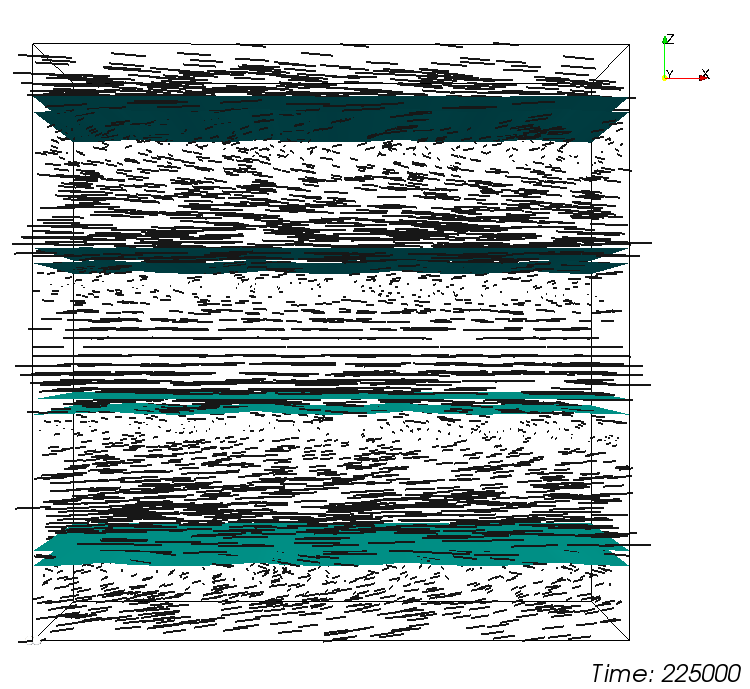
\includegraphics[width=0.5\textwidth]{dir-op-y_225k_run949.png}
\caption{BPII at high shear rate: director field and the disclination planes seen along the flow direction. The BPII breaks up and flows in helical layers separated from each other by a disclination plane}
\label{fig5}
\end{figure}

\subsection{Blue Phase I}

The flow behaviour of BPI deviates significantly from that of BPII in a number of points.
First of all it takes considerably longer to reach the steady state with periodically recurring patterns.
This might be because the disclination network of BPI undergoes much more complex flow-induced transformations than that of BPII.
Fig. \ref{fig6} shows a sequence of typical conformations at the same shear rate as Fig. \ref{fig1}, but this time seen along the direction of flow.
A similar affine transformation in flow-gradient plane takes place, which is however obscurred by the transformations shown here. 
The initial and final state in this sequence correspond to half a cycle. 
This can be easily verified by comparing the position of the disclination network at the left or right boundary.
BPI and BPII have exactly the same recurrence period, although it is seemingly four times shorter if the travelling of the network in z-direction is not taken into account.  

\begin{figure*}[h]
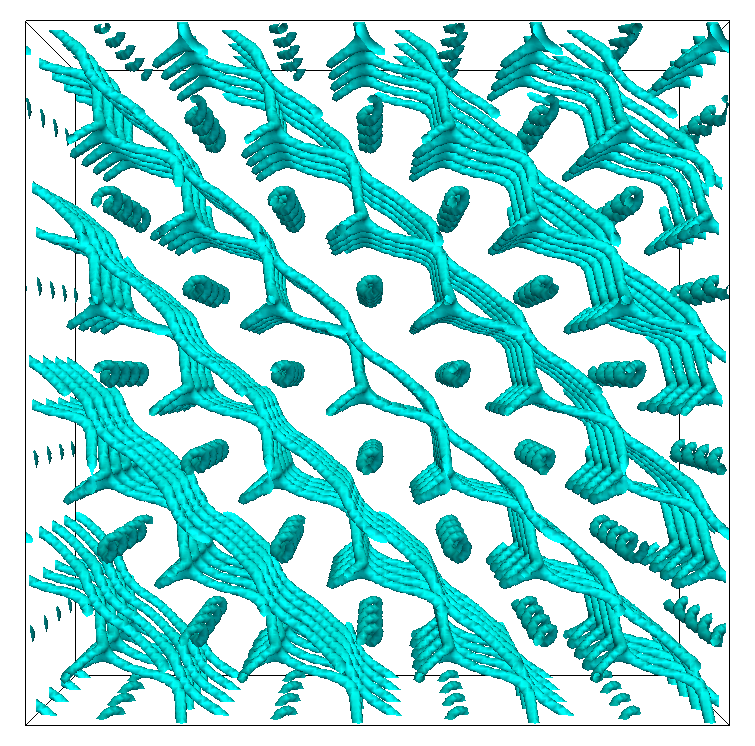
\includegraphics[width=0.32\textwidth]{disc-365k_run914.png}
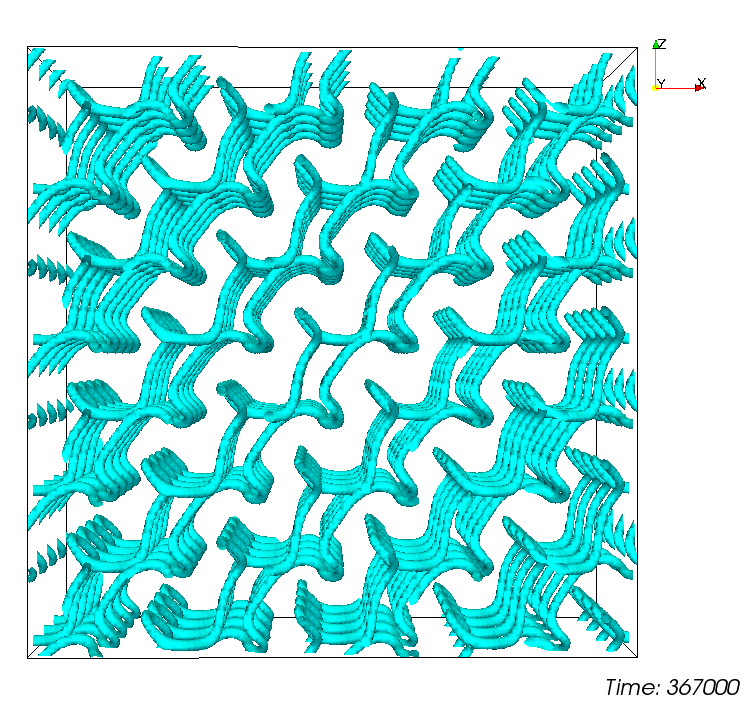
\includegraphics[width=0.32\textwidth]{disc-367k_run914.png}
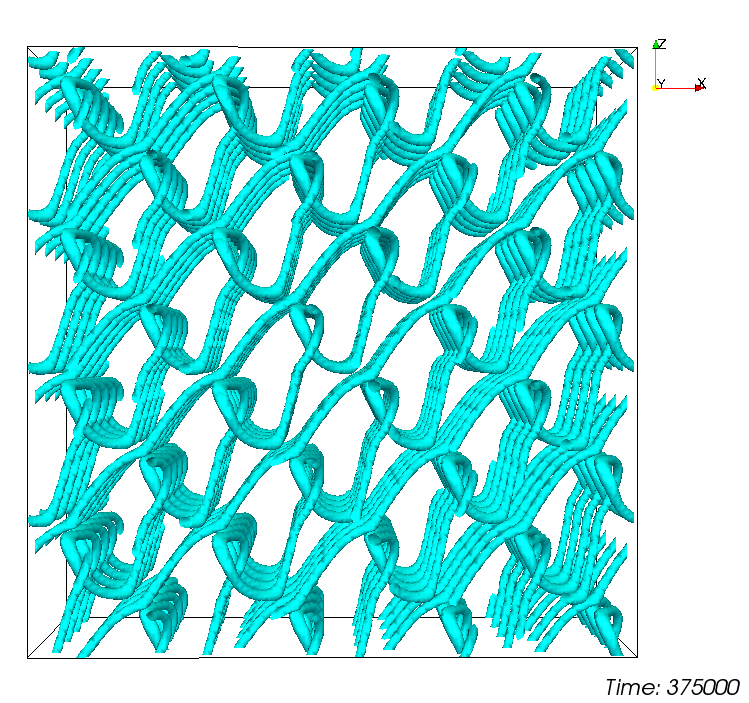
\includegraphics[width=0.32\textwidth]{disc-375k_run914.png}\\
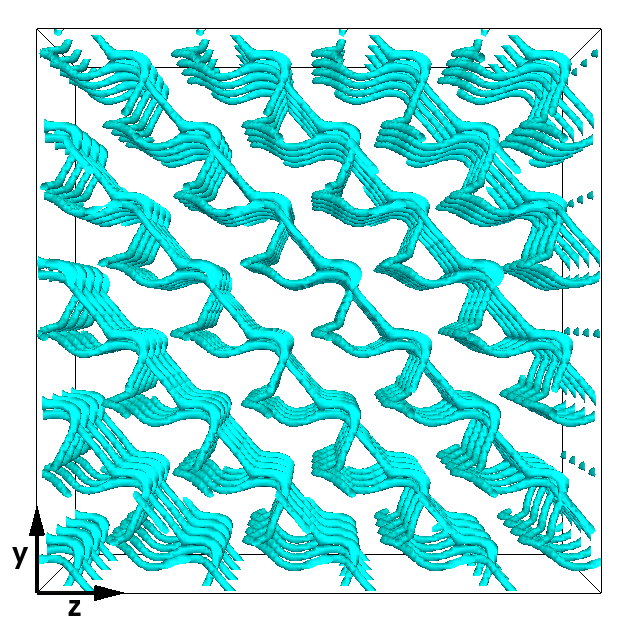
\includegraphics[width=0.32\textwidth]{disc-380k_run914.png}
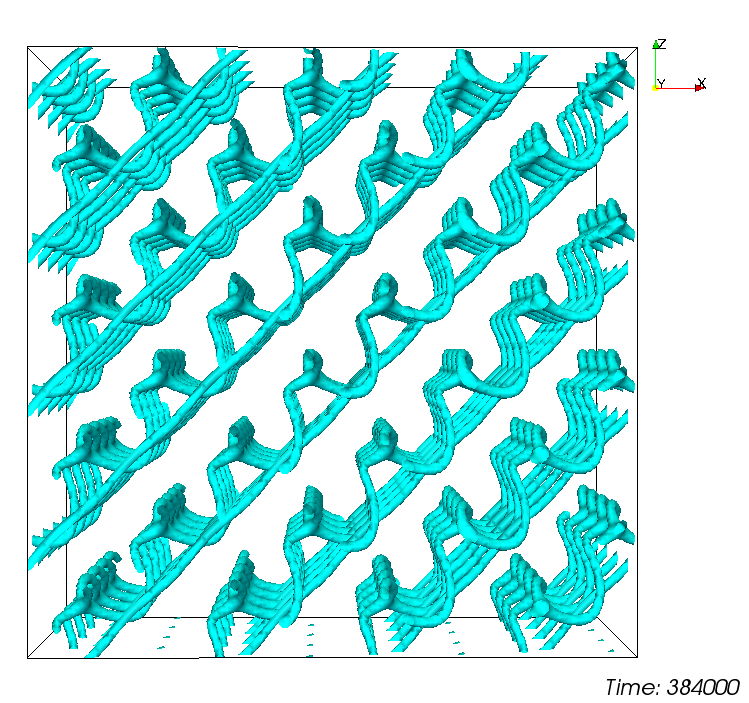
\includegraphics[width=0.32\textwidth]{disc-384k_run914.png}
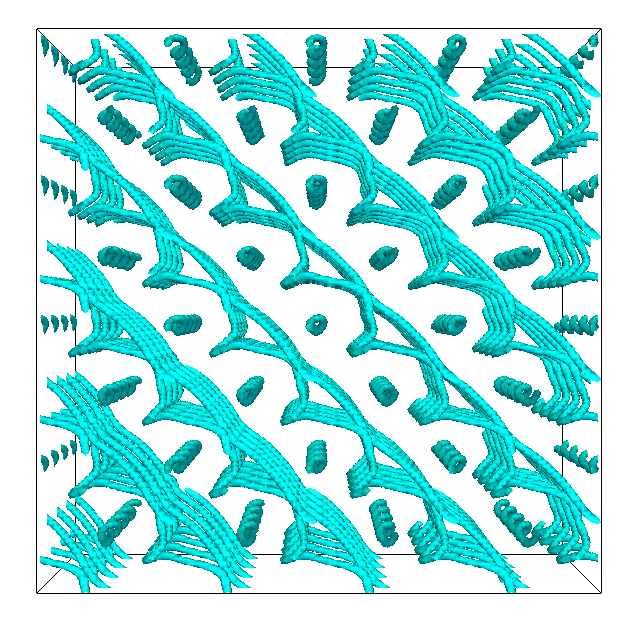
\includegraphics[width=0.32\textwidth]{disc-389k_run914.png}
\caption{Disclination network of BPI seen along the flow direction in steady shear flow at $\dot{\gamma}=1.56\cdot 10^{-4}$, showing the downward movement of the disclination network in the direction of vorticity.}
\caption{\label{fig6}}
\end{figure*}

The disclination network and the x- and z-component of the flow velocity are depicted in Fig. \ref{fig7}.
Just as in the previous case of BPII inverting the helix in the initial configuration inverts the sense of motion of the network in z-direction.
Equally it leads to an inversion of the velocities, shown here for a particular time steps, but due to the different topology and the complicated conformational changes there is no simple band structure as previously observed for BPII. 

\begin{figure*}[h]
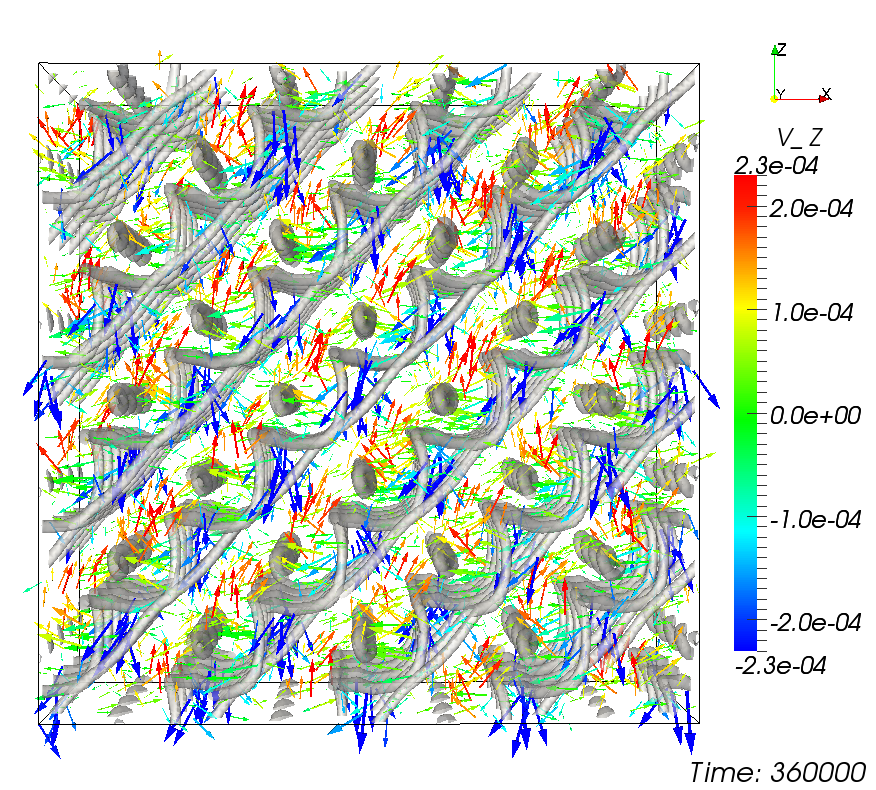
\includegraphics[width=0.45\textwidth]{v_xz-v_z-360k_run914.png}
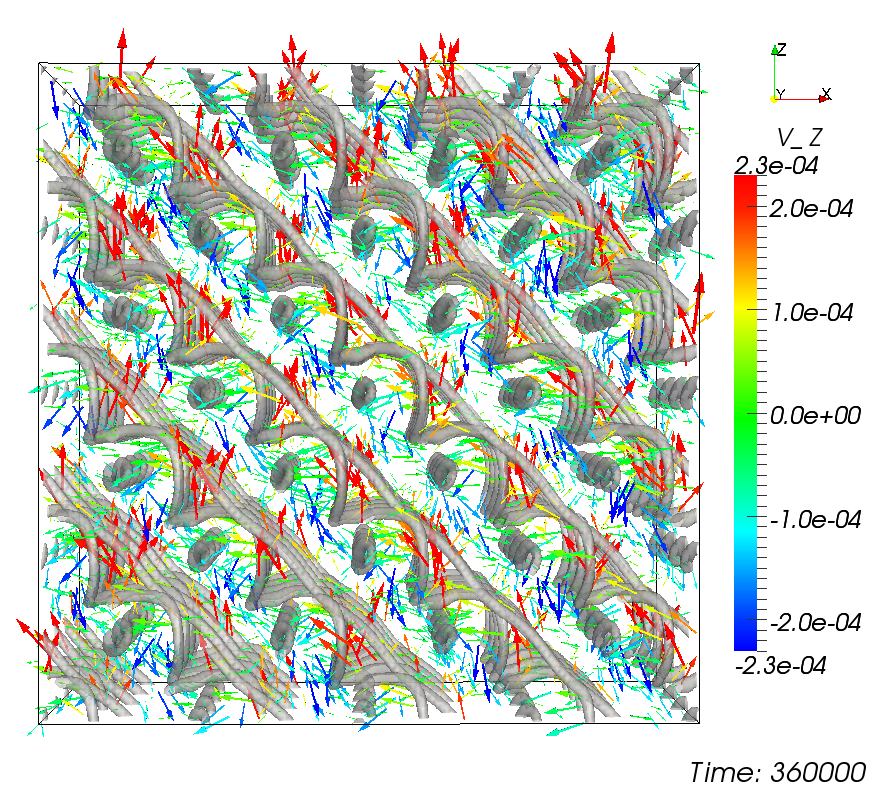
\includegraphics[width=0.45\textwidth]{v_xz-v_z-360k_run922.png}
\caption{Secondary flow in BPI: velocity components $v_x$ and $v_z$ for positive (left) and negative (right) helicity.}
\label{fig7}
\end{figure*}

Despite qualitative similarities between the BPI and BPII, the quantitative analysis reveals striking differences.
In Fig. \ref{fig8} we show the effective viscosity $\eta_{eff}$ over time and flow curves $\sigma_{chem}(\dot{\gamma})$. 
BPI exhibits pronounced shear-thinning contrary to BPII, whereas the shape of the curves in no longer symmetric.
In fact on approaching the critical shear rate that led in the case of BPII to the disruption of the network, the curves become increasingly complex but remain fully periodic.
The effective viscosity drops by about an order of magnitude between the lowest and the highest shear rates.
Note that the scale has been adapted to allow for the different magnitudes.
The inset can be directly compared with that of Fig. \ref{fig4}.
Interestingly the difference between minima and maxima of the chemical shear stress is much larger than for BPII and for the lowest shear rate we applied the absolute minimum takes even negative values, which are not shown in Fig. \ref{fig4}.
Our understanding of this phenomenon is an interplay of the elastic forces and the individual order paramter configuration of the liquid crystal.
If the system is close to a local minimum of the free energy but moving away from it the increasing strain pumps elastic energy into the system. 
This results in positive chemical stresses as the system tries to withstand the deformation.
However, if the system has sufficiently transformed and is about to overcome a local maximum, it will be pulled towards the next local minumum, which can lead temporarily to negative chemical stresses. 
The inset shows that the chemical stress decreases monotonically with decreasing flow rate, but does not follow a simple power law dependence.
 
\begin{figure}[h]
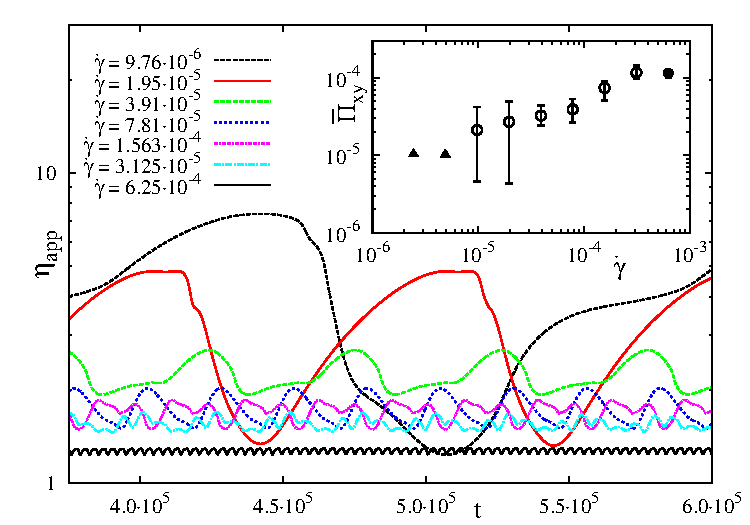
\includegraphics[width=0.5\textwidth]{stress_bp1.pdf}
\caption{Effective viscosity $\eta_{eff}=\Sigma_{xy}/\dot{\gamma}$ over time and flow curve $\sigma_{chem}(\dot{\gamma})$ (inset) of BPI in the steady state.}
\label{fig8}
\end{figure}

A Fourier analysis of the time series of the deviatoric chemical stress $\sigma_{eff,xy}$ or alternatively the free energy density $f$ can provide a further insight into the flow behaviour of BPI.
Fig. \ref{fig9} shows the Fourier spectrum of the time series of the chemical stress.
For simplicity we have always doubled the shear rate, so that the first overtone ocoalesces with the fundamental mode of the next highest shear rate. 
At low shear rates we observe a strong contribution of the first harmonic, which is directly related to the recurrence period $T$, shear rate $\dot{\gamma}$ and unit cell size $l_{u}$ via $\omega_0=2\pi/T=2\pi/(l_{u}\dot{\gamma})$.
The magnitude of higher harmonics decreases monotonously with increasing frequency.
Interestingly the inset of Fig. \ref{fig9} shows that at intermediate shear rates the contribution of higher harmonics becomes more pronounced until after a kind of gap and similar break up the fundamental mode dominates again and the former characteristics are restored.
Remarkably the break up in case of BPI occurs in exactly the same flow rate window as BPII.

\begin{figure}[h]
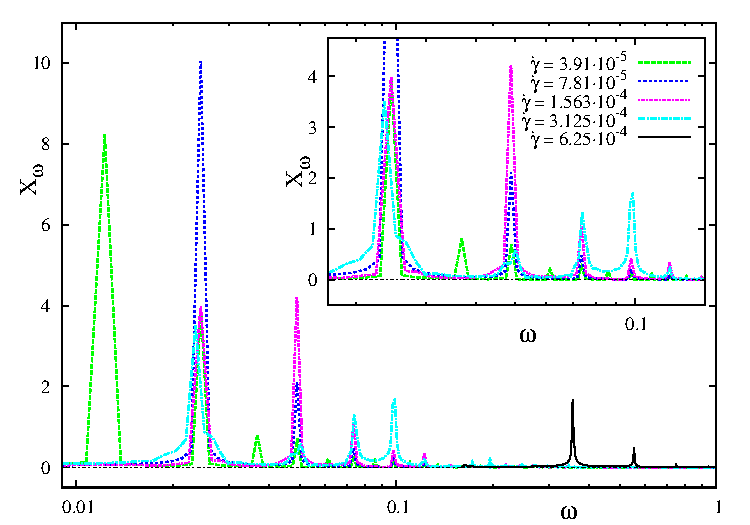
\includegraphics[width=0.5\textwidth]{spectrum_bp1.pdf}
\caption{Spectrum of the time series of the chemical stress over time. The frequency is given in units of $10^2\cdot 2\pi/T$ whereas $T$ is the recurrence period in LB time steps.}
\label{fig9}
\end{figure}

Nevertheless, the disclination network and order parameter strucutre of both phases looks strikingly different in this high flow rate state.
Fig. \ref{fig10} shows a snapshot along the gradient direction and the direction of vorticity.
Contrary to BPII BPI forms rolls which are advected by the flow and undergo a simple affine transformation similar to that of BPII below the break up point.
They meet in $\pm\pi/2$ disclinations, which are oriented along the z-direction.

\begin{figure}[h]
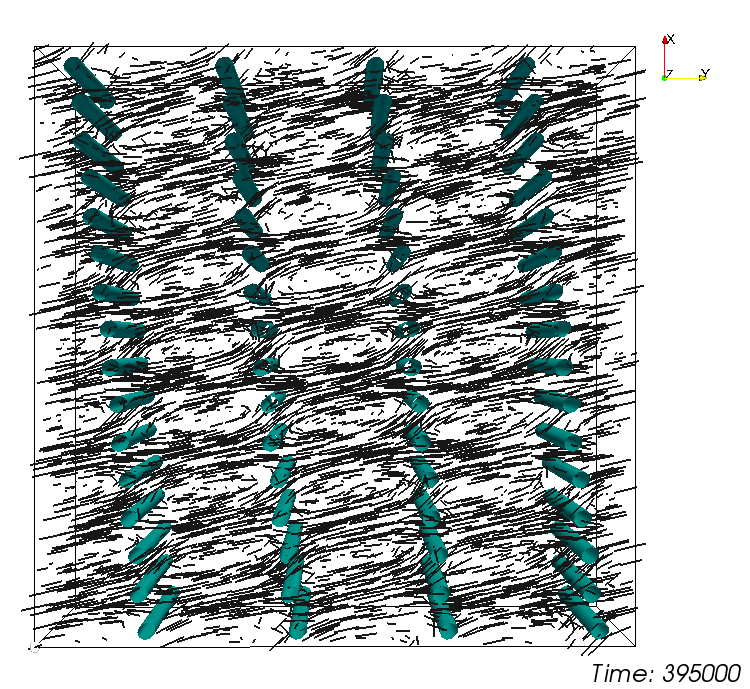
\includegraphics[width=0.5\textwidth]{dir-op-z_395k_run916.png}
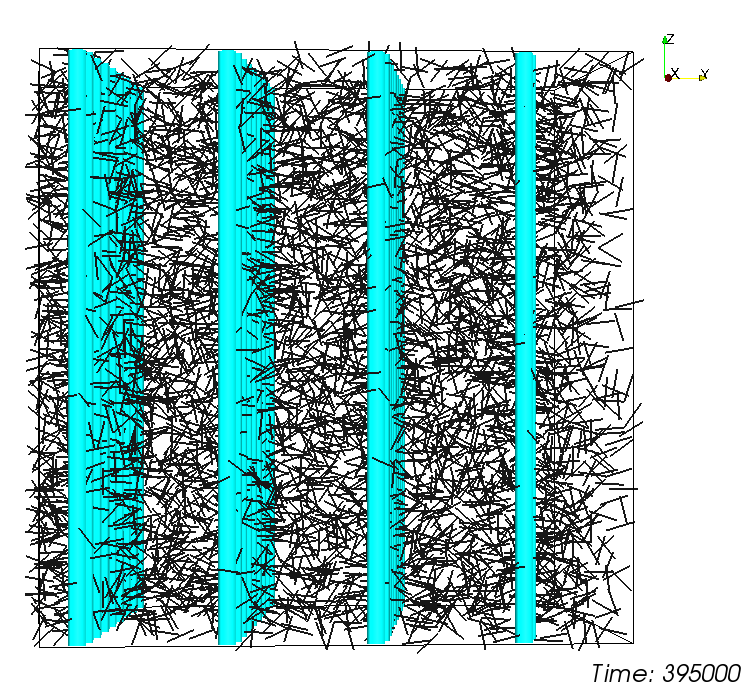
\includegraphics[width=0.5\textwidth]{dir-op-x_395k_run916.png}
\caption{BPI at high shear rate: director field and the disclination planes seen along the direction of voritcity and the gradient direction. BPI forms rolls with $\pi/2$ disclinations that are advected with the general flow.}
\label{fig10}
\end{figure}


\section{Conclusions}

% If in two-column mode, this environment will change to single-column
% format so that long equations can be displayed. Use
% sparingly.
%\begin{widetext}
% put long equation here
%\end{widetext}

% figures should be put into the text as floats.
% Use the graphics or graphicx packages (distributed with LaTeX2e)
% and the \includegraphics macro defined in those packages.
% See the LaTeX Graphics Companion by Michel Goosens, Sebastian Rahtz,
% and Frank Mittelbach for instance.
%
% Here is an example of the general form of a figure:
% Fill in the caption in the braces of the \caption{} command. Put the label
% that you will use with \ref{} command in the braces of the \label{} command.
% Use the figure* environment if the figure should span across the
% entire page. There is no need to do explicit centering.

% \begin{figure}
% \includegraphics{}%
% \caption{\label{}}
% \end{figure}

% Surround figure environment with turnpage environment for landscape
% figure
% \begin{turnpage}
% \begin{figure}
% \includegraphics{}%
% \caption{\label{}}
% \end{figure}
% \end{turnpage}

% tables should appear as floats within the text
%
% Here is an example of the general form of a table:
% Fill in the caption in the braces of the \caption{} command. Put the label
% that you will use with \ref{} command in the braces of the \label{} command.
% Insert the column specifiers (l, r, c, d, etc.) in the empty braces of the
% \begin{tabular}{} command.
% The ruledtabular enviroment adds doubled rules to table and sets a
% reasonable default table settings.
% Use the table* environment to get a full-width table in two-column
% Add \usepackage{longtable} and the longtable (or longtable*}
% environment for nicely formatted long tables. Or use the the [H]
% placement option to break a long table (with less control than 
% in longtable).
% \begin{table}%[H] add [H] placement to break table across pages
% \caption{\label{}}
% \begin{ruledtabular}
% \begin{tabular}{}
% Lines of table here ending with \\
% \end{tabular}
% \end{ruledtabular}
% \end{table}

% Surround table environment with turnpage environment for landscape
% table
% \begin{turnpage}
% \begin{table}
% \caption{\label{}}
% \begin{ruledtabular}
% \begin{tabular}{}
% \end{tabular}
% \end{ruledtabular}
% \end{table}
% \end{turnpage}

% Specify following sections are appendices. Use \appendix* if there
% only one appendix.
\appendix*

\begin{table*}
\begin{tabular}{|c|| c | c| c || c |c |c||c| c| c||c| c| c|}
\hline
$\dot{\gamma}$ & $\tau$ & $\kappa$ & $q_0$ & $\bar{v}_{x,min}$ & $\bar{v}_{x,max}$ & $\bar{v}_{x,std}$ & $\bar{v}_{y,min}$ & $\bar{v}_{y,max}$ & $\bar{v}_{y,std}$ & $\bar{v}_{z,min}$ & $\bar{v}_{z,max}$ & $\bar{v}_{z,std}$ \\
\hline
BPI \\
\hline
1.95 & -0.5 & 1.0 &0.1388 & -2.49 &2.50 &4.51 &-124.65 &124.82 &3.62 &-1.62 &1.89 &3.51 \\
3.91 & -0.5 & 1.0 &0.1388 & -3.31 &3.35 &4.21 &-248.69 &248.74 &3.90 &-2.88 &2.56 &4.39 \\
7.81 & -0.5 & 1.0 &0.1388 &-6.49 &6.56 &7.99 &-497.22 &496.16 &4.46 &-7.46 &5.31 &6.81 \\ 
15.63 & -0.5 & 1.0 &0.1388 &-3.08 &3.17 &10.49 &-992.46 &993.18 &10.36 &-3.57 &2.87 &10.54 \\
15.63 & -0.5 & 1.0 &-0.1388 &-3.08 &3.17 &10.49 &-992.46 &993.18 &10.36 &-2.87 &3.57 &10.54 \\
31.25 & -0.5 & 1.0 &0.1388 &-4.08 &4.46 &15.94 & -1988.36 &1986.71 &16.85 &-12.16 &11.37 &19.38\\
62.50 & -0.5 & 1.0 &0.1388 & -62.63 & 62.13 & 24.68 & -4039.41 &3995.3  & 20.57 &-110.76  &73.52 & 33.26 \\
\hline
BPII \\
\hline
1.95 & -0.5 & 2.0 & 0.1963 & -1.09 &1.07 & 0.76 &  -62.04  &61.60 & 0.97 & -1.55 &1.64 & 0.81\\
3.91 & -0.5 & 2.0 & 0.1963&-1.66 &1.70 & 1.45 &-123.93 &123.18 & 1.76 &-2.73 &3.09 &1.47\\
7.81 &  -0.5 & 2.0 &0.1963& -2.62 &2.71 & 2.67 &-247.67 &246.45 & 3.20 &-4.77 &5.78 &2.74\\
15.63 & -0.5 & 2.0 & 0.1963&-3.13 &3.31 &4.24 &-494.85 &493.09 & 5.64 &-7.66 &10.00 &4.33\\
15.63 & -0.5 & 2.0 &-0.1963& -3.13 &3.31 &4.24 &-494.85 &493.09 & 5.64 &-10.00 &7.66 &4.33\\
31.25 & -0.5 & 2.0 &0.1963 &-1.79 &1.82 &5.86 &-988.73 &985.93 &8.96  &-11.04 &14.39 &6.35\\
62.50 & -0.5 & 2.0 &0.1963 & -1.20 & 1.20 & 0.38 & -1969.41  & 1969.41 & 3.07 &-1.48 &0.96 &0.38 \\
\hline
\end{tabular}
\caption{Time-averaged velocity components in shear flow: Given are minumum and maximum values in $10^{-5}$ lattice units and the maximum standard deviation over the entire time sequence excluding transient dynamics, which means times t$\ge$200000 for BPI and t$\ge$30000 in case of BPII.
\label{table1}}
\end{table*}
%\section{}

% If you have acknowledgments, this puts in the proper section head.
\begin{acknowledgments}
Thanks folks!
\end{acknowledgments}

% Create the reference section using BibTeX:
\bibliography{bprheo}

\end{document}
%
% ****** End of file apstemplate.tex ******

